\subsection{Possible Explanations for Gender Differences}

\textbf{[JJH: Way too much emphasis on CBA.][We changed this section to focus on the treatment effects.] [JJH: We need the moderation and mediator analyses.]}

These treatment effects point to gender differences but do not explain the mechanisms through which they occur. An important factor at play is the issue of alternative preschool. There are substantial differences between males and females in one counterfactual: treatment vs. alternative preschools. The estimated treatment effects are very similar across genders for treatment compared to those staying at home full time. Males benefit much more from treatment relative to alternative preschools compared to their benefits from treatment relative to staying at home. This result is consistent with findings noted elsewhere: (i) stark gender differences resulting from attending low quality childcare \citep{Kottelenberg-Lehrer_2014_Gender-Effects,Baker_Gruber_Milligan_2015_Noncog_Defects}; and (ii) females are less sensitive to uncertain environments (see, e.g., \citealp{Autor-etal_2015_Family-Disadvantage}).

In Figure~\ref{fig:value-added}, we show the gender differences between subjects in the full control group and conditioning on different alternative care (home or lower quality center care). For early sociability, although females in the full control group have slightly higher scores, the males in the control group that stayed at home surpass the females by about 8 quantiles (out of 30 quantiles). These males even surpass the treatment-group males, which is why the value added of treatment is negative in this case. This is consistent with the parenting measures in which the control-group males outperform the other groups.

In addition to a gender difference in alternative preschool experiences, there are gender differences in the experience of ABC/CARE treatment. We analyze this by looking at the specific effects of the intervention on parenting.\footnote{In this exercise, we use We use measurements of the Home Observation for Measurement of the Environment (HOME; \citet{Bradley-Caldwell_1977_AJMD}). Although the exact scales vary by age, the scales of the HOME measure generally measure maternal warmth and involvement, absence of punishment, provision of appropriate toys, encouragement of mature behavior and independence, and the physical and language environment. The full score is the sum of these scales.}

When graphing the density of a factor combining the parenting skills measured at different ages, the density of the treatment group in both the male and female subsamples is bimodal (Figure~\ref{fig:total-home}). Because this is not the case for the control group, it is possible that treatment is moderated by another input of home environment. We consider the input of father's presence because it is highly correlated with selection into alternative preschool. For males, the mean of the treatment group if the father is present is greater than that of the treatment group if the father is absent. The reverse is seen for the females.

\begin{figure}
\textbf{[JJH: We need many more parenting measures.]}
\begin{center}
\caption{Density of the HOME Scores by Gender and Experimental Group}
\label{fig:total-home}

	\begin{subfigure}[b]{0.49\textwidth}
		\centering
		\caption{Parenting Skills, Males}
		\label{fig:home-male-factor}
			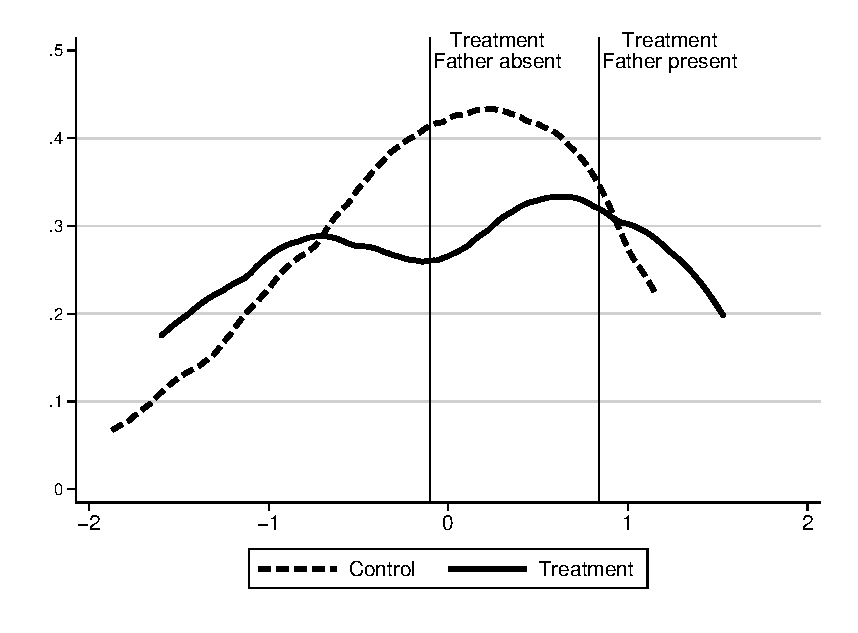
\includegraphics[width=\textwidth]{output/HOME-males-factorhome}
	\end{subfigure}
	\begin{subfigure}[b]{0.49\textwidth}
		\centering
		\caption{Parenting Skills, Females}
		\label{fig:home-female-factor}
			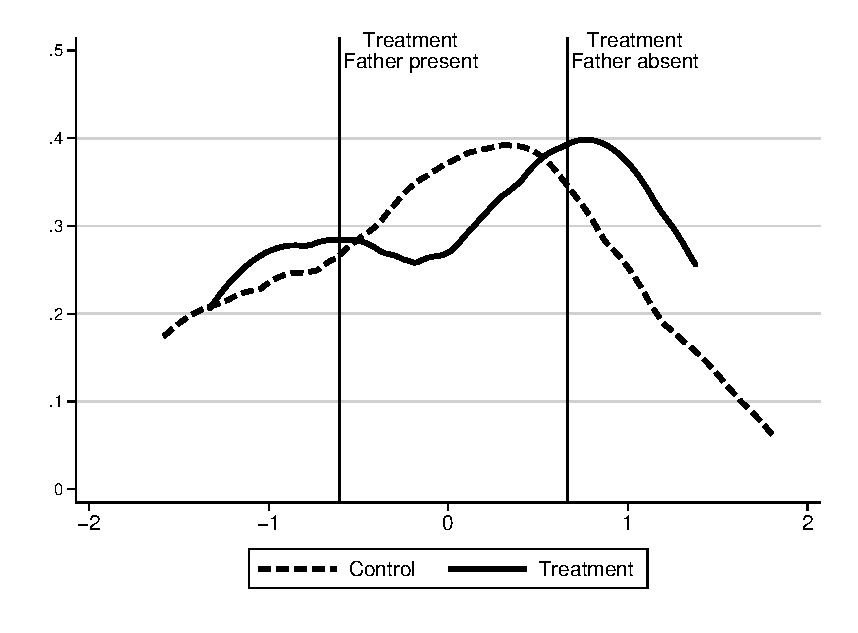
\includegraphics[width=\textwidth]{output/HOME-females-factorhome}
	\end{subfigure}
\end{center}
\raggedright
Note: These plots show the distribution the factor of HOME scores. The factors are computed by gender using full HOME scores at 0.5, 1.5, 2.5, and 8 years. The vertical lines are the means of the treatment group by father's presence.
\end{figure}

We explore this trend more closely in Figure~\ref{fig:total-home-quantiles}. To do so, we calculate the distribution pooling experimental groups but splitting by gender and father's presence. We then calculate, by gender and father's presence, the proportion of the treatment group that is in quantile 1 versus quantile 2. We do the same for the control group.

\begin{sidewaysfigure}
\begin{center}
\caption{Factor HOME Scores}
\label{fig:total-home-quantiles}
	\begin{subfigure}[b]{0.49\textwidth}
		\centering
		\caption{HOME, Father Absent, Males}
		\label{fig:home-male-mean}
			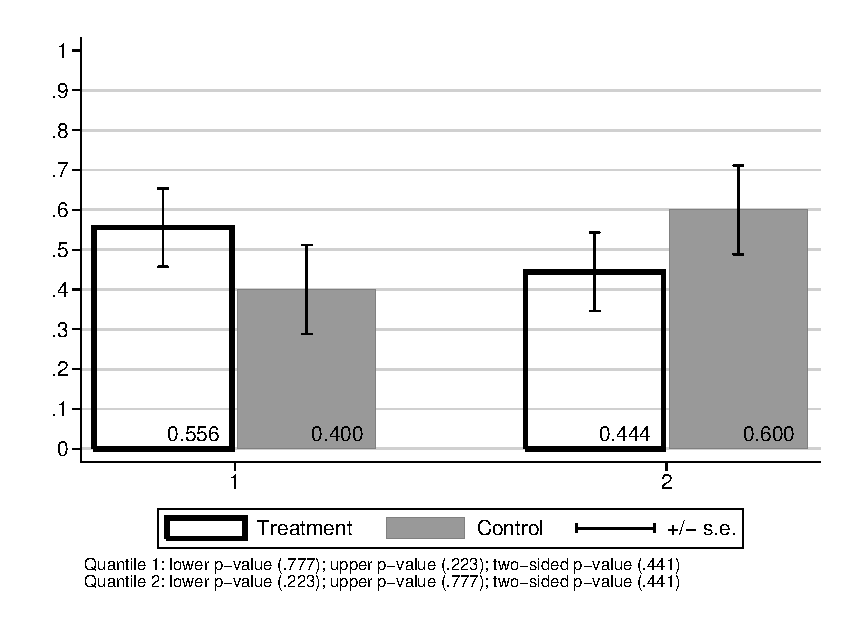
\includegraphics[width=\textwidth]{output/HOME-male1-fhome0-2quant}
	\end{subfigure}
	\begin{subfigure}[b]{0.49\textwidth}
		\centering
		\caption{HOME, Father Absent, Females}
		\label{fig:home-female-mean}
			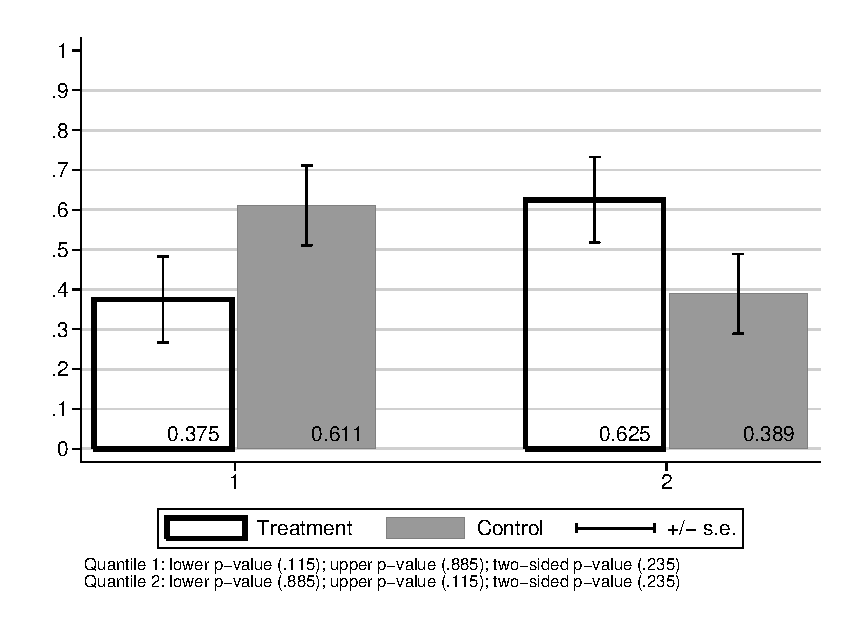
\includegraphics[width=\textwidth]{output/HOME-male0-fhome0-2quant}
	\end{subfigure}
	
	\begin{subfigure}[b]{0.49\textwidth}
		\centering
		\caption{HOME, Father Present, Males}
		\label{fig:home-male-factor}
			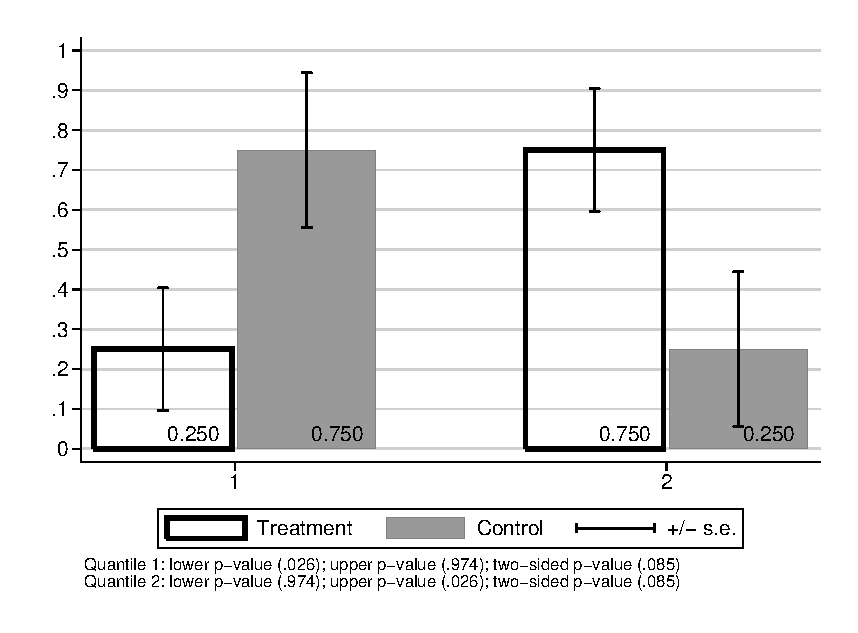
\includegraphics[width=\textwidth]{output/HOME-male1-fhome1-2quant}
	\end{subfigure}
	\begin{subfigure}[b]{0.49\textwidth}
		\centering
		\caption{HOME, Father Present, Females}
		\label{fig:home-female-factor}
			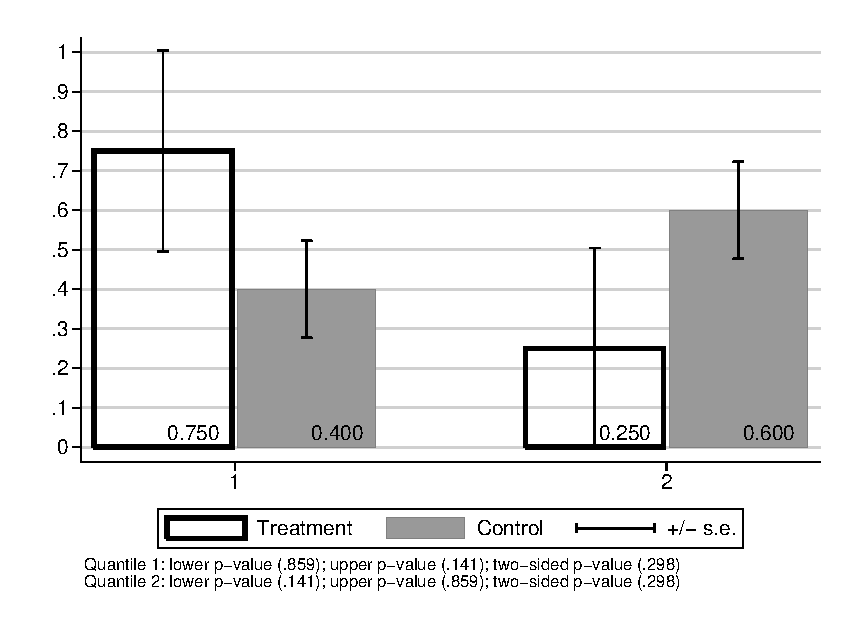
\includegraphics[width=\textwidth]{output/HOME-male0-fhome1-2quant}
	\end{subfigure}
\end{center}
\raggedright \footnotesize
Note: The horizontal axis divides a factor of the HOME scores into the first and second quantile of the distribution pooling across experimental groups, but splitting  by gender and father's presence. The factors are computed by gender using full HOME scores at 0.5, 1.5, 2.5, and 8 years. The lower $p$-value tests that the treatment proportion is less than the control proportion within a quantile. The upper $p$-value tests that the treatment proportion is greater than the control proportion within a quantile. The numbers reported in the bars are the proportions. All standard errors and $p$-values are calculated using 1,000 bootstraps.
\end{sidewaysfigure}

The result of this exercise shows that the bimodal shape of the densities of the treatment group is explained differently by gender. For males, the parenting measures are higher for the control group when the fathers are absent and higher for the treatment group when father's are present. For females, the opposite is the case: The parenting measures are higher for the control group when fathers are present and higher for the treatment group when fathers are absent.


\textbf{[JJH: Report results for controls (see comment 7a \& 7b). We need to deemphasize CBA. We are spoiling its market.][We have edited this section to discuss the gender differences in the treatment effects and the moderators and the control substitution. We will continue to add to this, including mediaiton.]}


